\graphicspath{{figures/tornado/}}
\chapter{龙卷风风场及其数值模拟}\label{chapter:tornado}

\section{龙卷风的特性及描述}
无论是模拟龙卷风,还是评估龙卷风对结构的影响,都需要对龙卷风的风场特性进行研究。
人们采用龙卷风的强度级数来衡量龙卷风造成的破坏的程度。
但由于龙卷风风场的复杂性,实际工程的抗龙卷风设计中,一般对其进行简化。
目前工程界主要通过给定龙卷风的特征参数以及通过Rankine涡模型中给定的龙卷风切向速度和压强等详细流场信息,来确定龙卷风对结构的影响。

\subsection{龙卷风的强度等级}
1970年,美国芝加哥大学的藤田(T. Theodore Fujita)教授提出将龙卷风按最大风速划分为7个等级,这种等级划分方法即为藤田级数。
但要直接测量龙卷风的最大风速并不容易,一般是根据龙卷风带来的破坏程度来估计龙卷风的最大风速,进而确定它的强度等级。

2007年2月1日起,美国气象部门采用改进的藤田级数(The Enhanced F-scale\cite{marshall2004enhanced})。
改进的藤田级数见表\ref{tab:EF_scale},分为EF0到EF5级。
它考虑了建筑物的坚固程度,对物体进行分类,共包括23种房屋以及5种非房屋类,如树木、桅杆等。
通过对给定各类物体的破坏描述,来估计龙卷风的最大风速,确定龙卷风的强度等级。
因此,改进的藤田级数能更准确地评估龙卷风的强度\cite{doswell2009implementation}。
\begin{table}[!htb]
	\caption{龙卷风强度级数的划分}
	\label{tab:EF_scale}
	\tabulinesep=2mm
	\centering
	%\begin{tabular*}{\textwidth}{c @{\extracolsep{\fill}} c p{11cm}}
	\begin{tabu} to 1.0\textwidth {X[1,c] X[2,c] X[6,l]}
		\toprule
		等级 & 风速(\SI{}{m/s}) & 破坏程度                                                                                                                                           \\ \midrule
		EF0    & $29.2-38.1$        & 轻度破坏:烟囱被损坏;刮断树枝;浅根系树木倾斜;毁坏商店招牌                                                             \\
		EF1    & $38.3-49.4$        & 中度破坏:掀起屋顶的砖瓦;掀翻移动住房;行动汽车被刮离路面                                                                \\
		EF2    & $49.7-60.6$        & 较严重破坏:刮走屋顶;摧毁活动住房;掀翻火车车厢;连根拔起大树;空中轻物乱飞;汽车被卷起                   \\
		EF3    & $60.8-73.9$        & 严重破坏:坚固房屋屋顶和墙壁被刮走;掀翻火车;森林中大多数树木被连根拔起;重型汽车被卷离地然后被抛起 \\
		EF4    & $74.2-89.4$        & 毁灭性破坏:坚固房屋被整体刮倒;基础不牢的建筑物被刮跑;汽车被抛向空中,空中比较大的物件横飞             \\
		EF5    & $>89.4$            & 极度破坏:坚固房屋框架被刮走;汽车大小的物件在空中横飞超过100米;飘飞碎片挂树梢;出现很罕见的现象       \\
		\bottomrule
		%\end{tabular*}
	\end{tabu}
\end{table}


\subsection{龙卷风的特征参数}
工程计算采用的龙卷风风场模型,具有如下参数:
(1)最大旋转风速$V_{\mathrm{R}}$;
(2)龙卷风涡的平移速度$V_{\mathrm{T}}$;
(3)最大旋转风速的半径$R$;
(4)气压降$\Delta P$;
(5)气压降速率$\mathrm{d} P/ \mathrm{d} t$。

我国《三十万千瓦压水堆核电厂安全重要土建结构抗龙卷风设计规定》中根据我国国情给出的两组龙卷风设计参数,如表\ref{tab:design_tornado}所示。除龙卷风发生概率低于$10^{-7}$的地区以外,根据厂址所在地区龙卷风资料的调研结果,从安全角度出发,选用一组合适的设计参数作为设计基准龙卷风\cite{EJ420-89}。
\begin{table}[!htbp]
	\caption{设计基准龙卷风特性}
	\label{tab:design_tornado}
	\centering
	%\begin{tabular*}{\textwidth}{c @{\extracolsep{\fill}} c c c c c c}
	\begin{tabu} to 1.0\textwidth {X[c] X[c] X[c] X[c] X[1.5,c] X[c] X[c] }
		\toprule
		组 & 最大风速     & 旋转风速                   & 平移风速                   & 最大旋转半径 & 压力降              & 降压时间   \\
		别 & $V (\SI{}{m/s})$ & $V_{\mathrm{R}}  (\SI{}{m/s})$ & $V_{\mathrm{T}}  (\SI{}{m/s})$ & $R (\SI{}{m})$     & $\Delta P (\SI{}{Pa})$ & $t (\SI{}{s})$ \\ \midrule
		A   & 107.3            & 84.9                           & 22.4                           & 45.7               & 8620                   & 2.5            \\
		B   & 134.1            & 107.3                          & 28.8                           & 45.7               & 13500                  & 1.875          \\ \bottomrule
	\end{tabu}
	%\end{tabular*}
\end{table}


\subsection{龙卷风的Rankine涡模型}
为了描述龙卷风风场的相关详细信息,工程界采用较多的是由Depperman\cite{Depperman1947}于1947年提出的Rankine涡模型。
Rankine涡模型是满足Navier-Stokes方程的最简单的模型,仅由切向速度控制。
它不考虑径向速度,并假定风速和压强不随高度变化,这在实际情况中是并不存在的。
但研究者最关心的也正是龙卷风的切向速度,因为相比于切向速度,龙卷风的径向速度和竖向速度较小。
其切向速度与离漩涡中心径向位置的关系曲线见图\ref{fig:Rankine}所示:强制涡区域内($r\leq R$)切向速度与半径成正比,而在自由涡区域内($r > R$)成反比。Rankine涡的切向速度表达式为\cite{Commission2007}:
\begin{equation}
	\label{eqn:Rankine}
	\begin{split}
		V_r &= \frac{r}{R} V_R,  \,\,\, r \leq R \\
		V_r &= \frac{R}{r} V_R,  \,\,\, r > R
	\end{split}
\end{equation}
式中:$V_r$是距涡中心为$r$处的切向风速,$V_{\mathrm{R}}$为Rankine涡中的最大切向风速,$R$为最大切向风速对应的旋转半径。
\begin{figure}[!htbp]
	\centering
	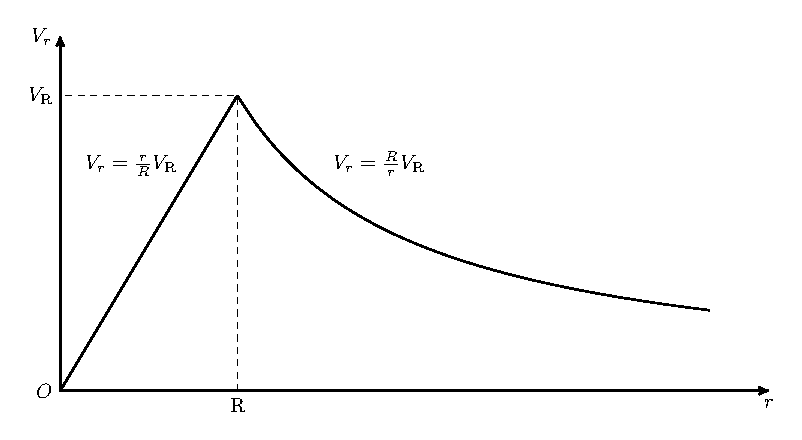
\includegraphics[width=0.6\textwidth]{Rankine.pdf}
	\caption{Rankine涡模型中切向速度沿涡半径的变化曲线图}
	\label{fig:Rankine}
\end{figure}


\section{缩尺龙卷风的CFD模拟}
本文选择Ward型龙卷风发生装置(Ward-type Tornado Vortex Chamber,下文简称Ward-TVC)\cite{ward1972exploration}的改进版(Purdue-TVC)\cite{church1979characteristics}进行数值模拟,Purdue-TVC的示意图见图\ref{fig:Ward-TVC}。
Davies-Jones\cite{davies1976laboratory}详细评述了各种龙卷风发生装置,认为Ward-TVC与实际发生的龙卷风之间具有较好的几何和动力学相似性(geometric and dynamic similarity)。

控制龙卷风风场的主要无量纲参数为\cite{lewellen1993tornado}:
高宽比$A$、涡流比$S$、雷诺数(Reynolds number)$\mathrm{Re}$、弗劳德数(Froude number)$\mathrm{Fr}=\left( \Delta P/ 2g\Delta \rho z\right)^{1/2}$;$\Delta P$为气压降、$\Delta \rho$为流域内空气密度的变化、$g$为重力加速度、$z$为距离地面的高度。
高宽比和涡流比的定义如下:
\begin{equation}
	A = H_0/R_0
\end{equation}
\begin{equation}
	S = V_t/2A V_r
\end{equation}
其中$R_0$为上升气流孔的半径,$H_0$为气流入口的高度(见图\ref{fig:Ward-TVC}),
$V_t$和$V_r$为$R_0$处的切向和径向入流速度。
试验\cite{ward1972exploration}\cite{church1979characteristics}\cite{snow1982review}和数值模拟\cite{davies1976laboratory}等说明涡流比是控制龙卷风风场特征的最主要参数。
图\ref{fig:swirl}展示了龙卷风风场结构随涡流比的增大而发生变化\cite{hangan2008swirl}。
\begin{figure}[!htbp]
	\centering
	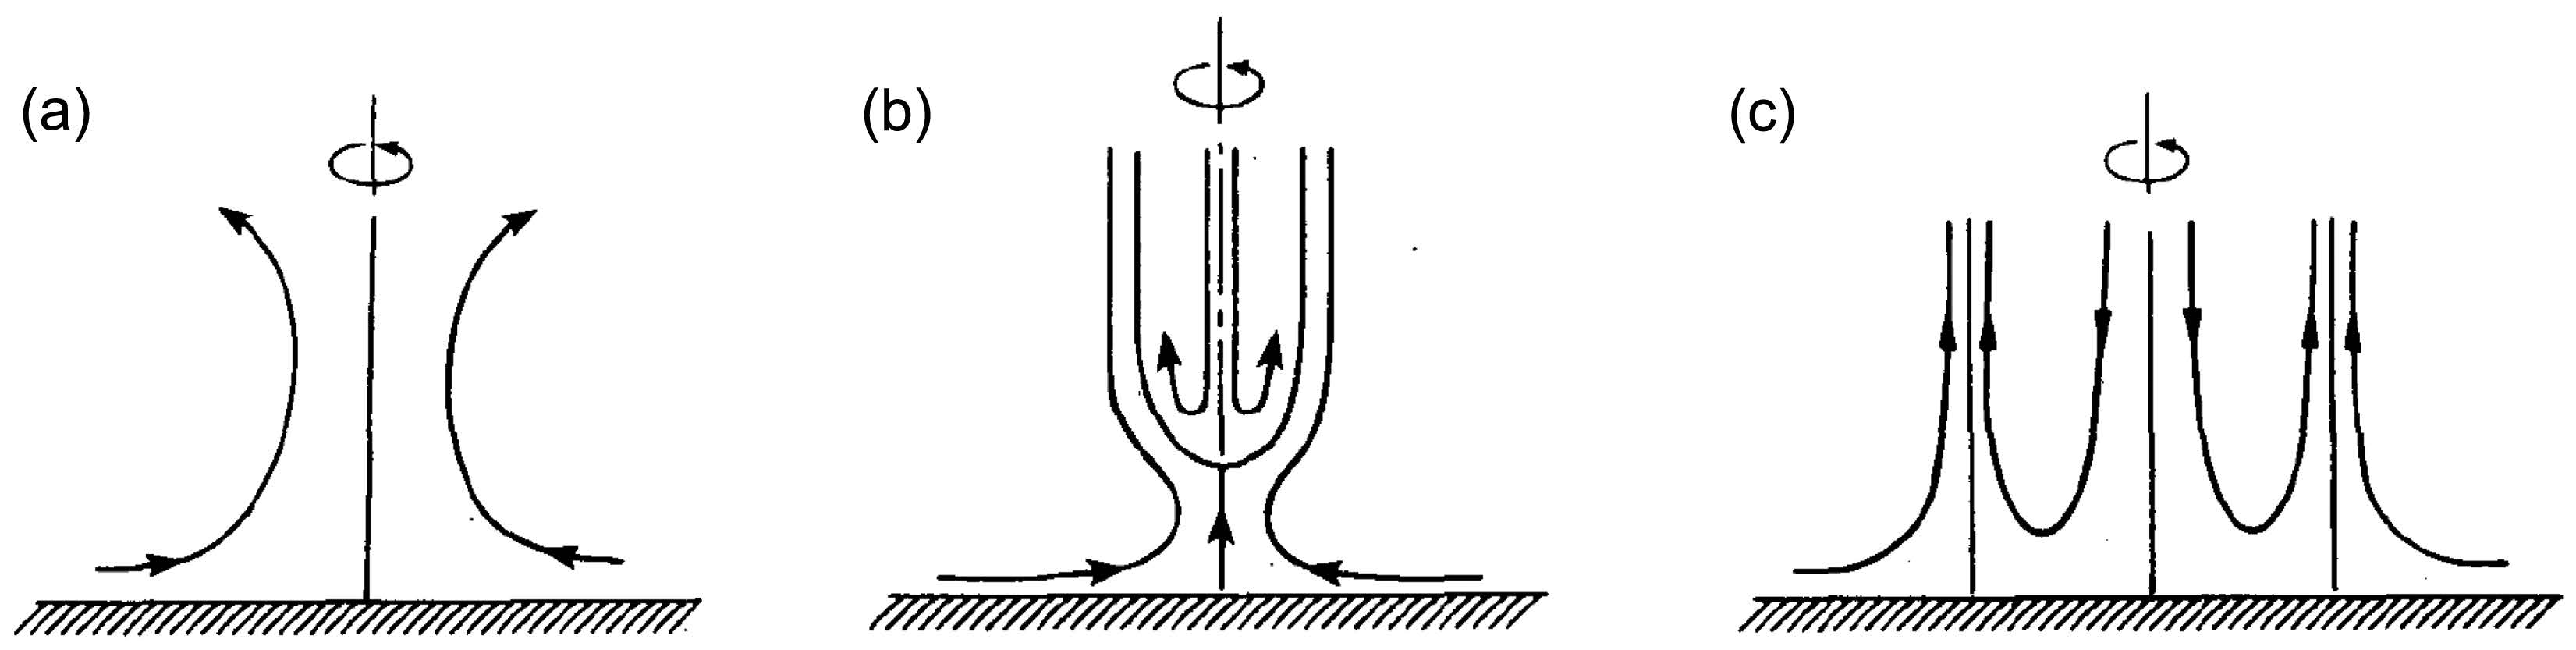
\includegraphics[width=\textwidth]{swirl_ratio_tornado_flow_pattern.jpg}
	\caption{增大涡流比引起龙卷风风场结构发生变化的示意图}\label{fig:swirl}
\end{figure}

随着涡流比的增大,龙卷风从射流状流场变化为单涡状涡旋(图\ref{fig:swirl}(a)),接着风场产生一个驻点、涡旋脱离地面(图\ref{fig:swirl}(b)),最后涡旋着地,分裂形成双涡状龙卷风(图\ref{fig:swirl}(c))。

本节主要介绍计算流体力学软件ANSYS Fluent模拟Ward-TVC的方法,并探讨涡流比对数值风场的影响。

\subsection{风场几何区域}
数值模拟的计算流域取Purdue-TVC的阴影区域,见图\ref{fig:Ward-TVC}。
为了与Baker\cite{baker1981boundary}的试验进行对比以验证数值风场的正确性,
取计算流域的尺寸及边界条件如图\ref{fig:tornado-domain}所示。
其中$X$轴对应龙卷风风场的径向,$Z$轴对应龙卷风风场的竖向。
\begin{figure}[!htbp]
	\begin{subfigure}[b]{0.5\textwidth}
		\centering
		\input{figures/tornado/Ward_TVC_sketch.pdf_tex}
		\caption{Purdue-TVC龙卷风发生装置示意图}\label{fig:Ward-TVC}
	\end{subfigure}
	\begin{subfigure}[b]{0.5\textwidth}
		\centering
		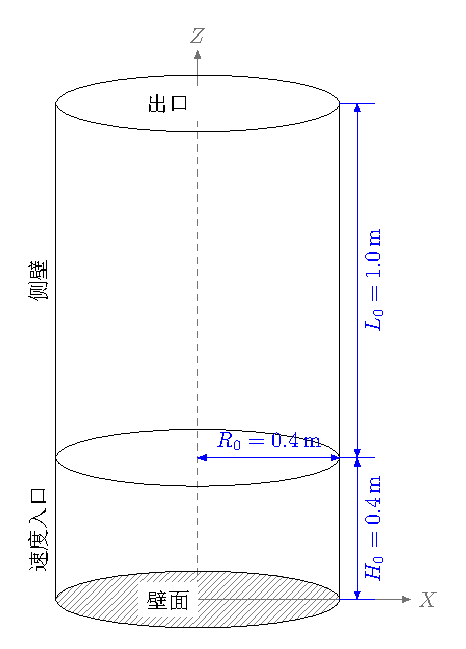
\includegraphics{domain.pdf}
		\caption{龙卷风数值模型的计算流域}\label{fig:tornado-domain}
	\end{subfigure}
	\caption{龙卷风发生装置和计算流域示意图}\label{fig:TVC-domain}
\end{figure}


\subsection{网格划分}
采用适应性良好的六面体结构化网格进行计算流域的划分。
初始网格数量大概为$300,000$,然后根据速度梯度和Y+进行自适应网格划分\cite{fluent2015user}。由于工程实际主要关注近地面附近龙卷风对结构的作用,
故细分主要针对近地面流域处的网格。不断加密网格直到近地面最大切向速度和最大切向速度所在半径的位置前后两次计算结果相差小于$5\%$。最后根据计算机的能力及计算结果的有效性,采用的网格数量为$1,536,000$。


\subsection{湍流模型}
龙卷风风场是旋流流场,根据Launder\cite{launder1989second}的研究,采用雷诺应力方程模型 (RSM)较为合适。
模型参数为:$C_{\mu}=0.09$; $C_{1\varepsilon}=1.44$; $C_{2\varepsilon}=1.92$; 
$C1-ps=1.8$; $C2-ps=0.6$; $C1'-ps=0.5$; $C2'-ps=0.3$。
湍流动能(TKE)普朗特数为 $1$; 湍动耗散率(TDR)普朗特数为 $1.3$。

\subsection{边界条件}
速度入口处径向和切向速度分布采用如下形式:
\begin{equation}\label{eqn:Vr}
	V_r(z) = V_0 \times (z/z_0)^{1/7}
\end{equation}
\begin{equation}\label{eqn:Vt}
	V_t(z) = 2 \times S \times V_r(z)
\end{equation}
式中,$V_r$为径向速度,$V_t$为切向速度,$V_0$为参考速度,$z_0$为参考高度,$S$为涡流比。

图\ref{fig:bc-inlet}为公式\eqref{eqn:Vr}和\eqref{eqn:Vt}所定义的风速分布与Baker\cite{baker1981boundary}试验的对比。
注意到试验风速分布与试验装置有关,而非实际的大气边界层风速分布。
公式\eqref{eqn:Vr}和\eqref{eqn:Vt}类似于大气边界层风速分布,并尽可能与Baker\cite{baker1981boundary}试验保持一致。
\begin{figure}[!htbp]
	\centering
	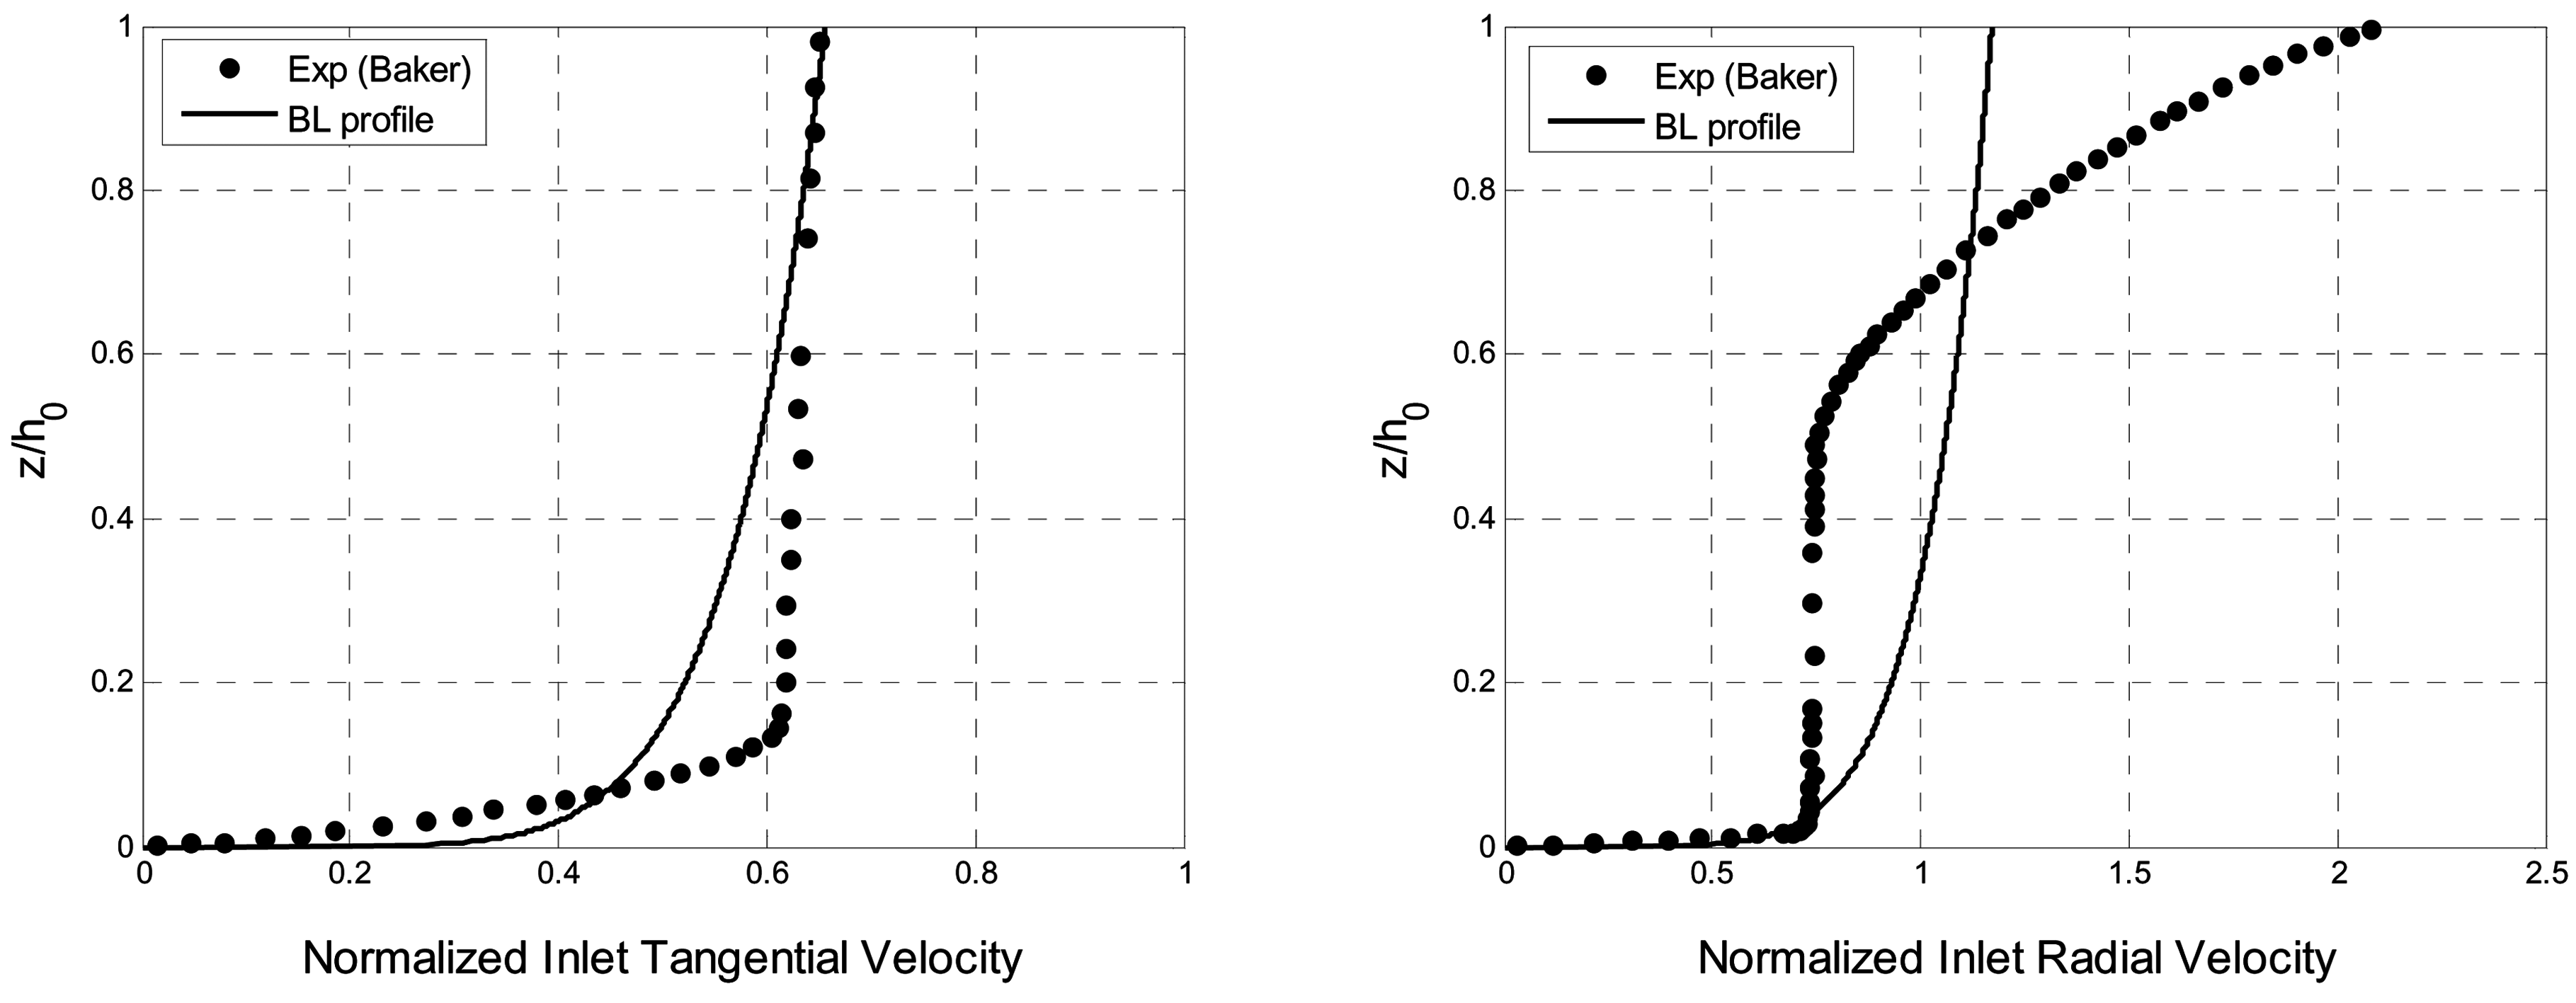
\includegraphics[width=\textwidth]{bc_inlet.png}
	\caption{入口处规格化切向和径向速度与Baker\cite{baker1981boundary}试验的对比}
	\label{fig:bc-inlet}
\end{figure}

试验表明,沿壁面法线方向的不同距离,可以将近壁面区域分成三层区域。
最里层,又称粘性底层,流动区域很薄,粘性力在动量、热量及质量交换中都起主导作用;
最外层为对数率层,粘性力不起主要作用;
两层之间的区域为过渡层,粘性力作用与湍流作用相当。

为描述粘性底层和对数率层内的流动,现引入无量纲参数$u^{+}$和$y^{+}$:
\begin{equation}
	u^{+} = \frac{u}{u_{\tau}}
\end{equation}
\begin{equation}
	y^{+} = \frac{y u_{\tau}}{\nu} = \frac{y}{\nu} \sqrt{\frac{\tau_w}{\rho}}
\end{equation}
式中:$u$是流体的时均速度、$u_{\tau}=\sqrt{\tau_w/\rho}$为壁面摩擦速度、$\tau_w$为壁面处切应力、$\nu$为空气动粘度系数、$y$为壁面第一层节点到壁面的距离。

以$y^{+}$的对数为横坐标,以$u^{+}$为纵坐标,可将壁面区域内的三个区域表示为图\ref{fig:uplus}所示\cite{fluent2015theory}。
\begin{figure}[!htbp]
	\centering
	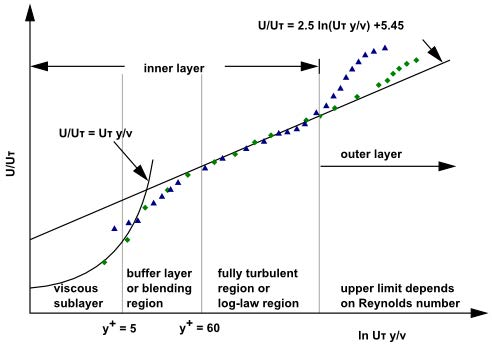
\includegraphics[width=0.6\textwidth]{figures/tornado/uplus.jpg}
	\caption{近壁面区域划分}\label{fig:uplus}
\end{figure}

通常有两种方法模拟近壁面区域:
一种采用“壁面方程”的半经验公式模拟受粘性力影响较大的区域,能够较好地修正湍流模型,解决壁面的存在对流场的影响;
另一种方法采用低$\mathrm{Re}$数的$k-\varepsilon$模型来求解粘性底层和过渡层,越靠近壁面,网格划分就越细,这种方法被称为“近壁面模型”法。
图\ref{fig:wall-treatment}为两种方法的对比\cite{fluent2015theory}。
\begin{figure}[!htbp]
	\centering
	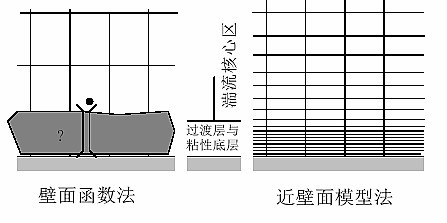
\includegraphics[width=0.8\textwidth]{wall_treatment.jpg}
	\caption{近壁面区域处理方法}
	\label{fig:wall-treatment}
\end{figure}

本文地面处采用强化壁面函数(Enhanced wall treatment\cite{fluent2015user}),需要对近壁面的网格进行细化。
边界层网格节点是否合适需要检查计算后的$y^{+}$值。
$y^{+}=u_{\tau} y/\nu$小于$1.5$能取得较好效果。

Smith的数值模拟\cite{smith1987effect}说明了侧壁的边界条件的选取对汇集区风场(主要关注的区域)的影响很小。
因此选择无滑壁面条件。

Purdue-TVC出口处设置了蜂窝板,能使气流竖直流出,还能阻止排风机对涡旋的影响。
试验中排风机驱动了流场运动,而在数值模型中,入口风速驱动了流场运动,且不包含排风机的影响,因此数值模型出口处不需设置代表直流蜂窝板的边界条件。根据Smith\cite{smith1987effect}的论述,上边界更合适的边界条件为压强出口边界条件(pressure-outflow)。
此边界条件假设除压强外的所有物理量在边界的法向梯度为零\cite{fluent2015user}。

\subsection{控制方程及求解选项}
控制方程采用非定常雷诺平均纳维-斯托克斯方程(Unsteady Reynolds Averaged Navier-Stokes, RANS)。
时间离散采用一阶隐性格式,压强速度场的耦合采用压力修正的分离式算法,SIMPLEC算法。
动量、TKE、TDR和雷诺应力采用二阶迎风格式。



\section{龙卷风数值模拟结果及其正确性验证}\label{sec:tornado}
图\ref{fig:tornado-domain}所示的风场几何区域,建立柱面坐标系$\{O:r \theta z\}$。
本文主要关注在柱面坐标系下数值风场的速度特征,其中径向(radial)、切向(tangential)、竖向(axial)风速分别记为$V_r(r,\theta,z)$、$V_t(r,\theta,z)$和$V_a(r,\theta,z)$。

考虑到龙卷风风场具有轴对称性,故对数值风场速度分布沿圆周($r=$常数)进行平均,消除速度随$\theta$的变化,得到轴对称的风场$V_r(r,z)$、$V_t(r,z)$和$V_a(r,z)$。

% 将上述轴对称风场与Baker试验\cite{baker1981boundary}结果及多普勒雷达实测风场进行对比,以验证数值风场的正确性。
% 并探讨缩尺龙卷风数值风场转化为足尺风场的方法。

\subsection{Baker试验对比}
Baker利用Purdue-TVC进行了龙卷风风场的试验模拟\cite{baker1981boundary},选取$S=0.28$的风场在$r/R_0=0.1025$和$r/R_0=0.2125$处风速各分量随高度变化曲线与数值风场进行对比。
将高度以$R_0$进行无量纲化,速度以入口平均径向速度$U_0=Q/(R_0 H_0)$进行无量纲化,其中$2\pi Q$为速度入口边界处的流量。
将\eqref{eqn:Vr}定义的速度入口边界的径向速度代入可得:
\begin{equation}
	U_0 = \frac{Q}{R_0 H_0} = \frac{R_0 \int_0^{H_0} V_r(z)\,\mathrm{d}z}{R_0 H_0} = \frac{\int_0^{H_0} V_0 (z/z_0)^{1/7}\,\mathrm{d}z}{H_0} = \frac{7}{8} V_0 \left(\frac{H_0}{z_0}\right)^{1/7}
\end{equation}

图\ref{fig:cfd_vs_exp_Vr}、图\ref{fig:cfd_vs_exp_Vt}和图\ref{fig:cfd_vs_exp_Va}分别为数值风场(CFD)与Baker试验无量纲化径向、切向和轴向风速随高度变化的对比图。
二者总体上吻合较好。

\begin{figure}[!htbp]
	\centering
	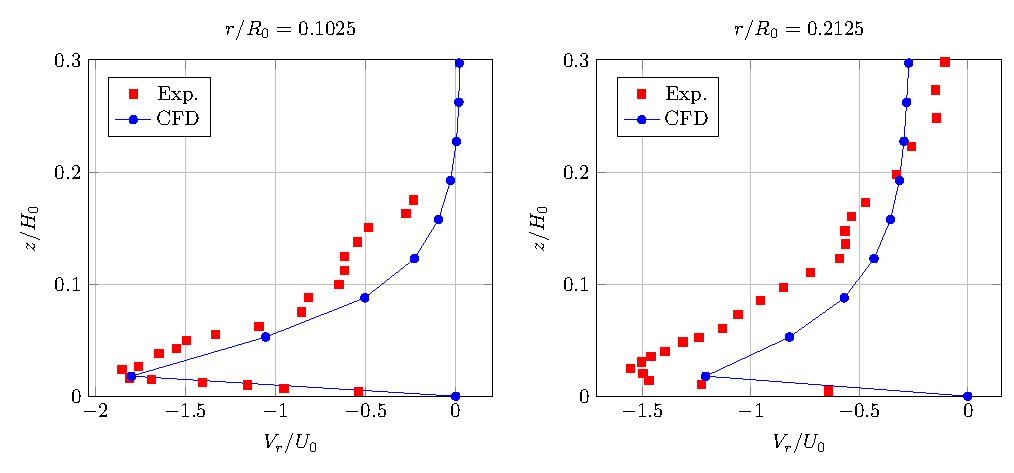
\includegraphics[width=1.0\textwidth]{cfd_vs_exp_Vr.pdf}
	\caption{数值风场与Baker试验无量纲化径向速度随高度变化的对比,$S=0.28$}
	\label{fig:cfd_vs_exp_Vr}
\end{figure}
\begin{figure}[!htbp]
	\centering
	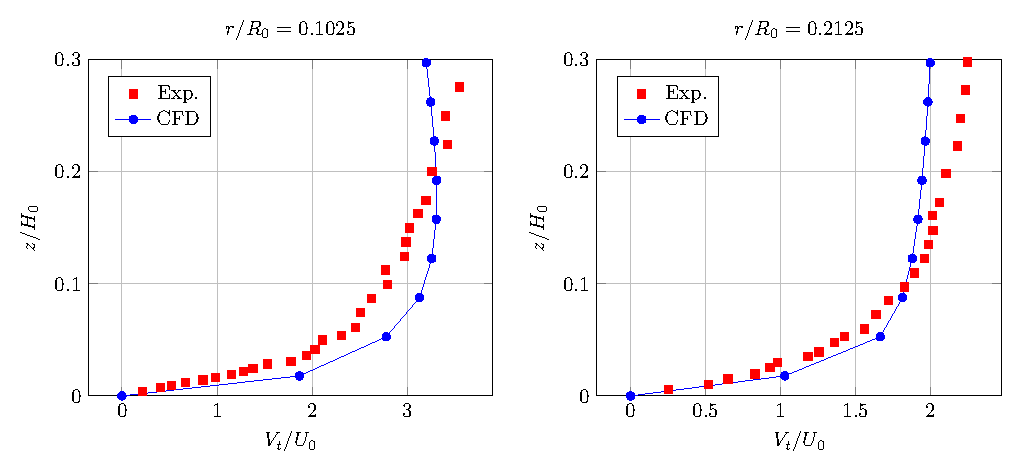
\includegraphics[width=1.0\textwidth]{cfd_vs_exp_Vt.pdf}
	\caption{数值风场与Baker试验无量纲化切向速度随高度变化的对比,$S=0.28$}
	\label{fig:cfd_vs_exp_Vt}
\end{figure}
\begin{figure}[!htbp]
	\centering
	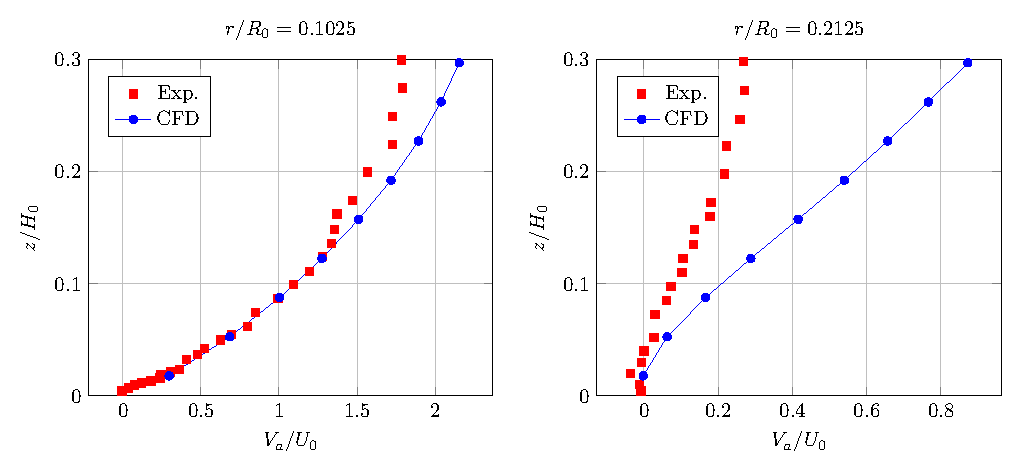
\includegraphics[width=1.0\textwidth]{cfd_vs_exp_Va.pdf}
	\caption{数值风场与Baker试验无量纲化竖向速度随高度变化的对比,$S=0.28$}
	\label{fig:cfd_vs_exp_Va}
\end{figure}

\subsection{数值风场的风速分布特征}
图\ref{fig:Vt-x=0}为计算流域轴向剖面($X=0$)处切向速度云图。
从图中可以明显看出涡旋中心处切向速度接近于零;
图\ref{fig:Vt-z=30mm}为\SI{30}{mm}高度处的切向速度云图,可以看出流域的涡旋接近中心轴线,并能显示出漏斗状形态,显示了龙卷风风场具有很好的涡旋特性。
由图\ref{fig:Vt}可知龙卷风涡旋中心的切向速度较小,在核心半径处达到最大,而后随着远离涡旋中心的距离增大而逐渐减小。
且在核心半径内,切向速度的变化较快,而远离核心半径时,变化逐渐缓和,与Rankine模型吻合较好。
此外还可看出随着离地高度的增加,核心半径有所增大,而最大切向风速呈逐渐减小的趋势。
\begin{figure}[!htbp]
	\begin{subfigure}[b]{0.5\textwidth}
		\centering
		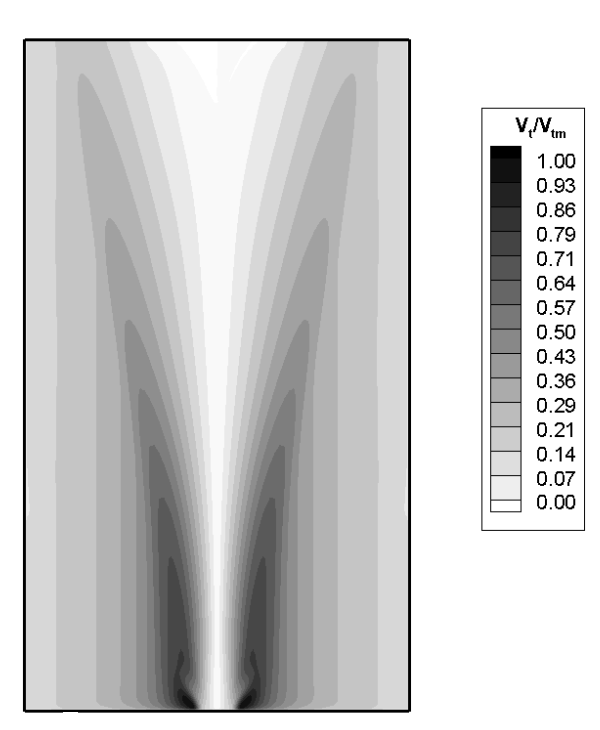
\includegraphics[width=\textwidth]{Vt_x=0.png}
		\caption{轴向剖面($X=0$)}\label{fig:Vt-x=0}
	\end{subfigure}
	\begin{subfigure}[b]{0.5\textwidth}
		\centering
		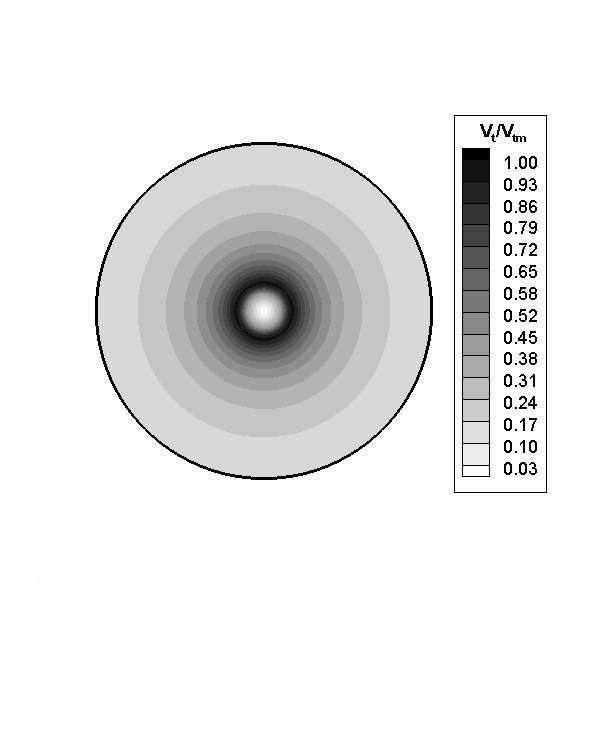
\includegraphics[width=\textwidth]{Vt_z=30mm.png}
		\caption{水平剖面($Z=\SI{30}{mm}$)}\label{fig:Vt-z=30mm}
	\end{subfigure}
	\caption{切向速度云图}\label{fig:Vt-contour}
\end{figure}

\begin{figure}
	\centering
	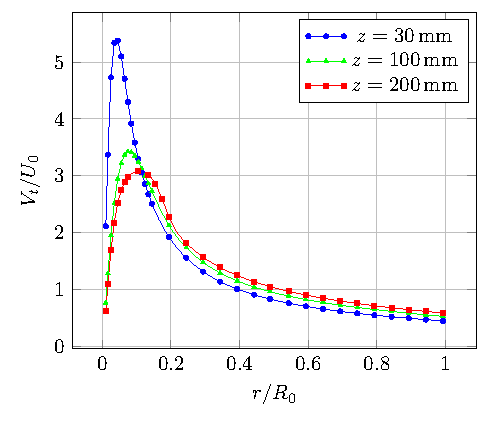
\includegraphics[width=0.6\textwidth]{Vt.pdf}
	\caption{数值风场不同高度处切向速度沿径向的变化图,$S=0.28$}
	\label{fig:Vt}
\end{figure}

\subsection{数值风场的风压分布特征}
图\ref{fig:P-x=0}和图\ref{fig:P-z=30mm}分别给出了计算流域轴向剖面($X=0$)和水平剖面($Z=\SI{30}{mm}$)处风压云图,$P_m$是风场最大静压,为负压。
可以看出龙卷风中心处离地面一定高度范围内存在很强的负压,且随着半径的增加而逐渐减小。

图\ref{fig:p}给出了三种不同高度处的风压沿径向的分布,可以看出不同高度处风压分布接近一致。

\begin{figure}[!htbp]
	\begin{subfigure}[b]{0.5\textwidth}
		\centering
		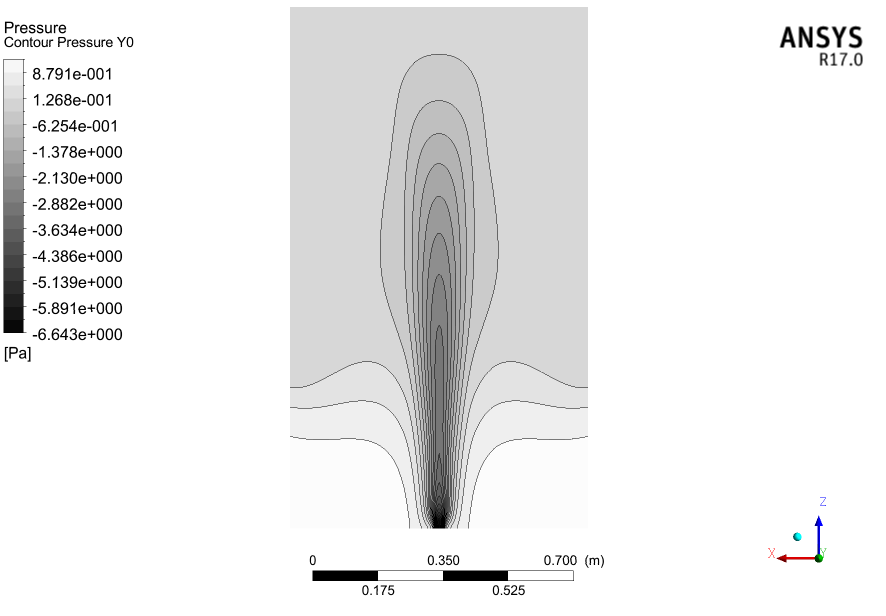
\includegraphics[width=\textwidth]{P_x=0.png}
		\caption{轴向剖面($X=0$)}\label{fig:P-x=0}
	\end{subfigure}
	\begin{subfigure}[b]{0.5\textwidth}
		\centering
		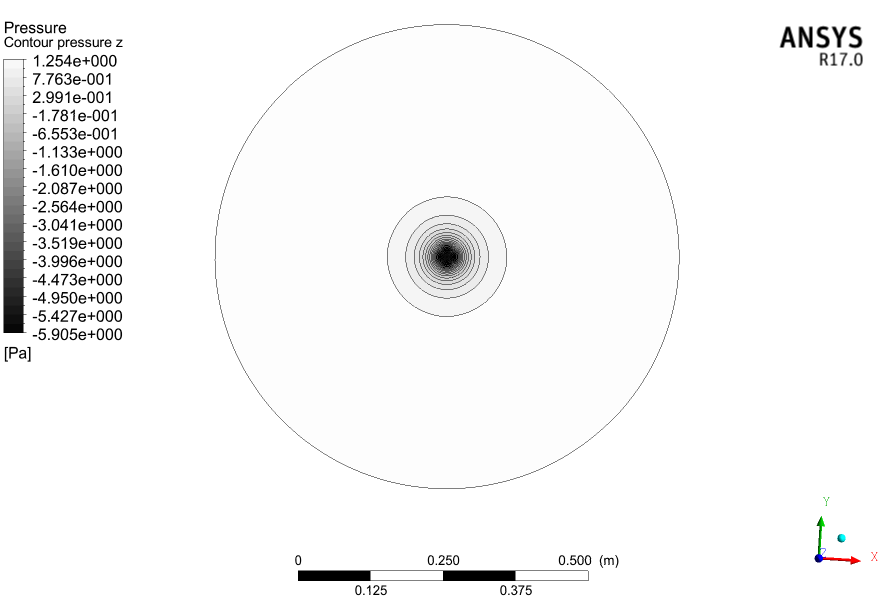
\includegraphics[width=\textwidth]{P_z=30mm.png}
		\caption{水平剖面($Z=\SI{30}{mm}$)}\label{fig:P-z=30mm}
	\end{subfigure}
	\caption{风压云图}\label{fig:p-contour}
\end{figure}

\begin{figure}[!htbp]
	\centering
	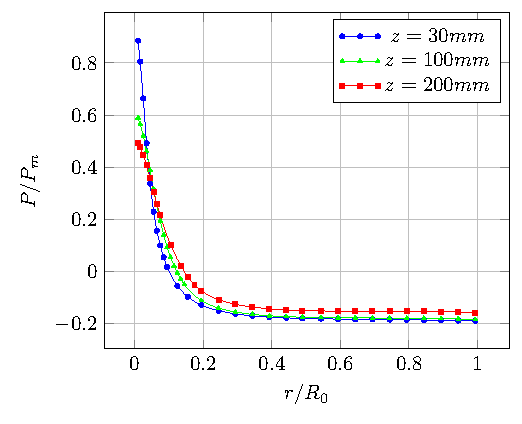
\includegraphics[width=0.6\textwidth]{p.pdf}
	\caption{数值风场不同高度处风压沿径向的变化图}
	\label{fig:p}
\end{figure}

\section{足尺龙卷风CFD模拟}

\subsection{长度相似比和速度相似比}

足尺风场选用1998年5月发生在美国南达科他州Spencer地区的实测龙卷风风场,
这些数据由车载式多普勒雷达采集,Wurman等人有详细的介绍\cite{wurman2002multiple}\cite{alexander2005spencer}\cite{wurman2005spencer}。

采集的风场在不同竖向高度处、\SI{2}{km}$\times$\SI{2}{km}的水平区域内(水平测点间距为\SI{20}{m})。
将原始风场去除龙卷风平移速度,得到涡旋风场,并利用最小二乘原理将速度场沿圆周平均,以消除多涡等因素的影响。
最终得到的龙卷风切向速度随离开涡旋中心径向距离的变化关系如图\ref{fig:Vt-full}所示。
\begin{figure}[!htbp]
	\centering
	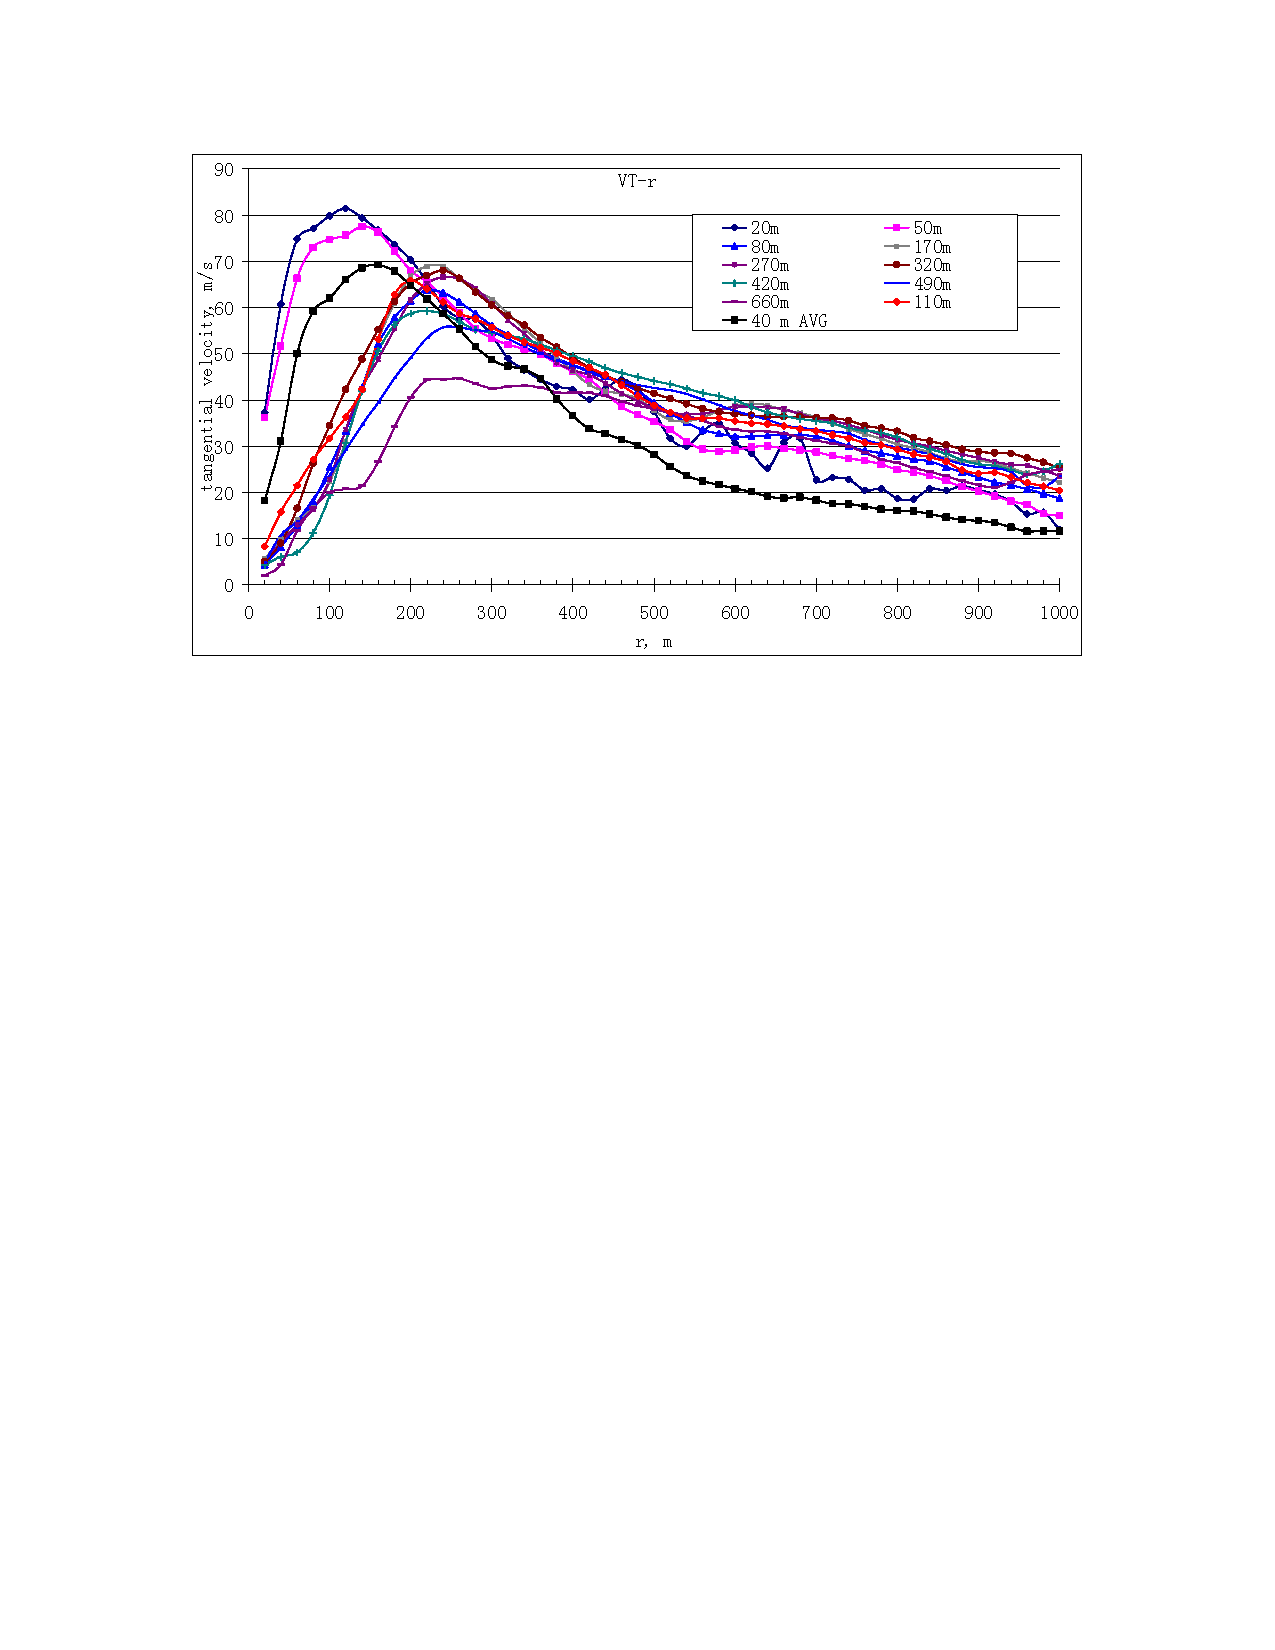
\includegraphics[width=0.8\textwidth]{Vt_full.pdf}
	\caption{实测风场在不同高度处切向速度与径向距离的关系曲线\cite{sarkar2005velocity}}
	\label{fig:Vt-full}
\end{figure}

考虑缩尺风场和实测风场的最大切向速度及其发生位置$V_t(r_{c\,\mathrm{max}}, z_{\mathrm{max}})$,
其中$r_{c,\mathrm{max}}$为风场在$z_{\mathrm{max}}$高度处的核心半径(龙卷风最大切向速度点距龙卷风中心的距离)。
速度相似比和长度相似比定义为\cite{hangan2008swirl}:
\begin{equation}
	V_s  =  \frac{V_{t,\mathrm{max}}^{\text{Full}}}{V_{t,\mathrm{max}}^{\text{CFD}}}
\end{equation}
\begin{equation}
	L_s  =  \frac{r_{c,\mathrm{max}}^{\text{Full}}}{r_{c,\mathrm{max}}^{\text{CFD}}} \quad \text{or} \quad \frac{z_{c,\mathrm{max}}^{\text{Full}}}{z_{c,\mathrm{max}}^{\text{CFD}}}
\end{equation}

本文模拟的缩尺龙卷风速度相似比为$V_s=60$。
文献\cite{hangan2008swirl}研究了长度相似比$L_s$随涡流比$S$变化的情况,见图\ref{fig:Ls-S}。
发现两种方式定义的长度相似比$L_s$随涡流比$S$的增大逐渐趋向于定值。
本文取长度相似比$L_s$为该定值$4000$。

\begin{figure}[!htbp]
	\centering
	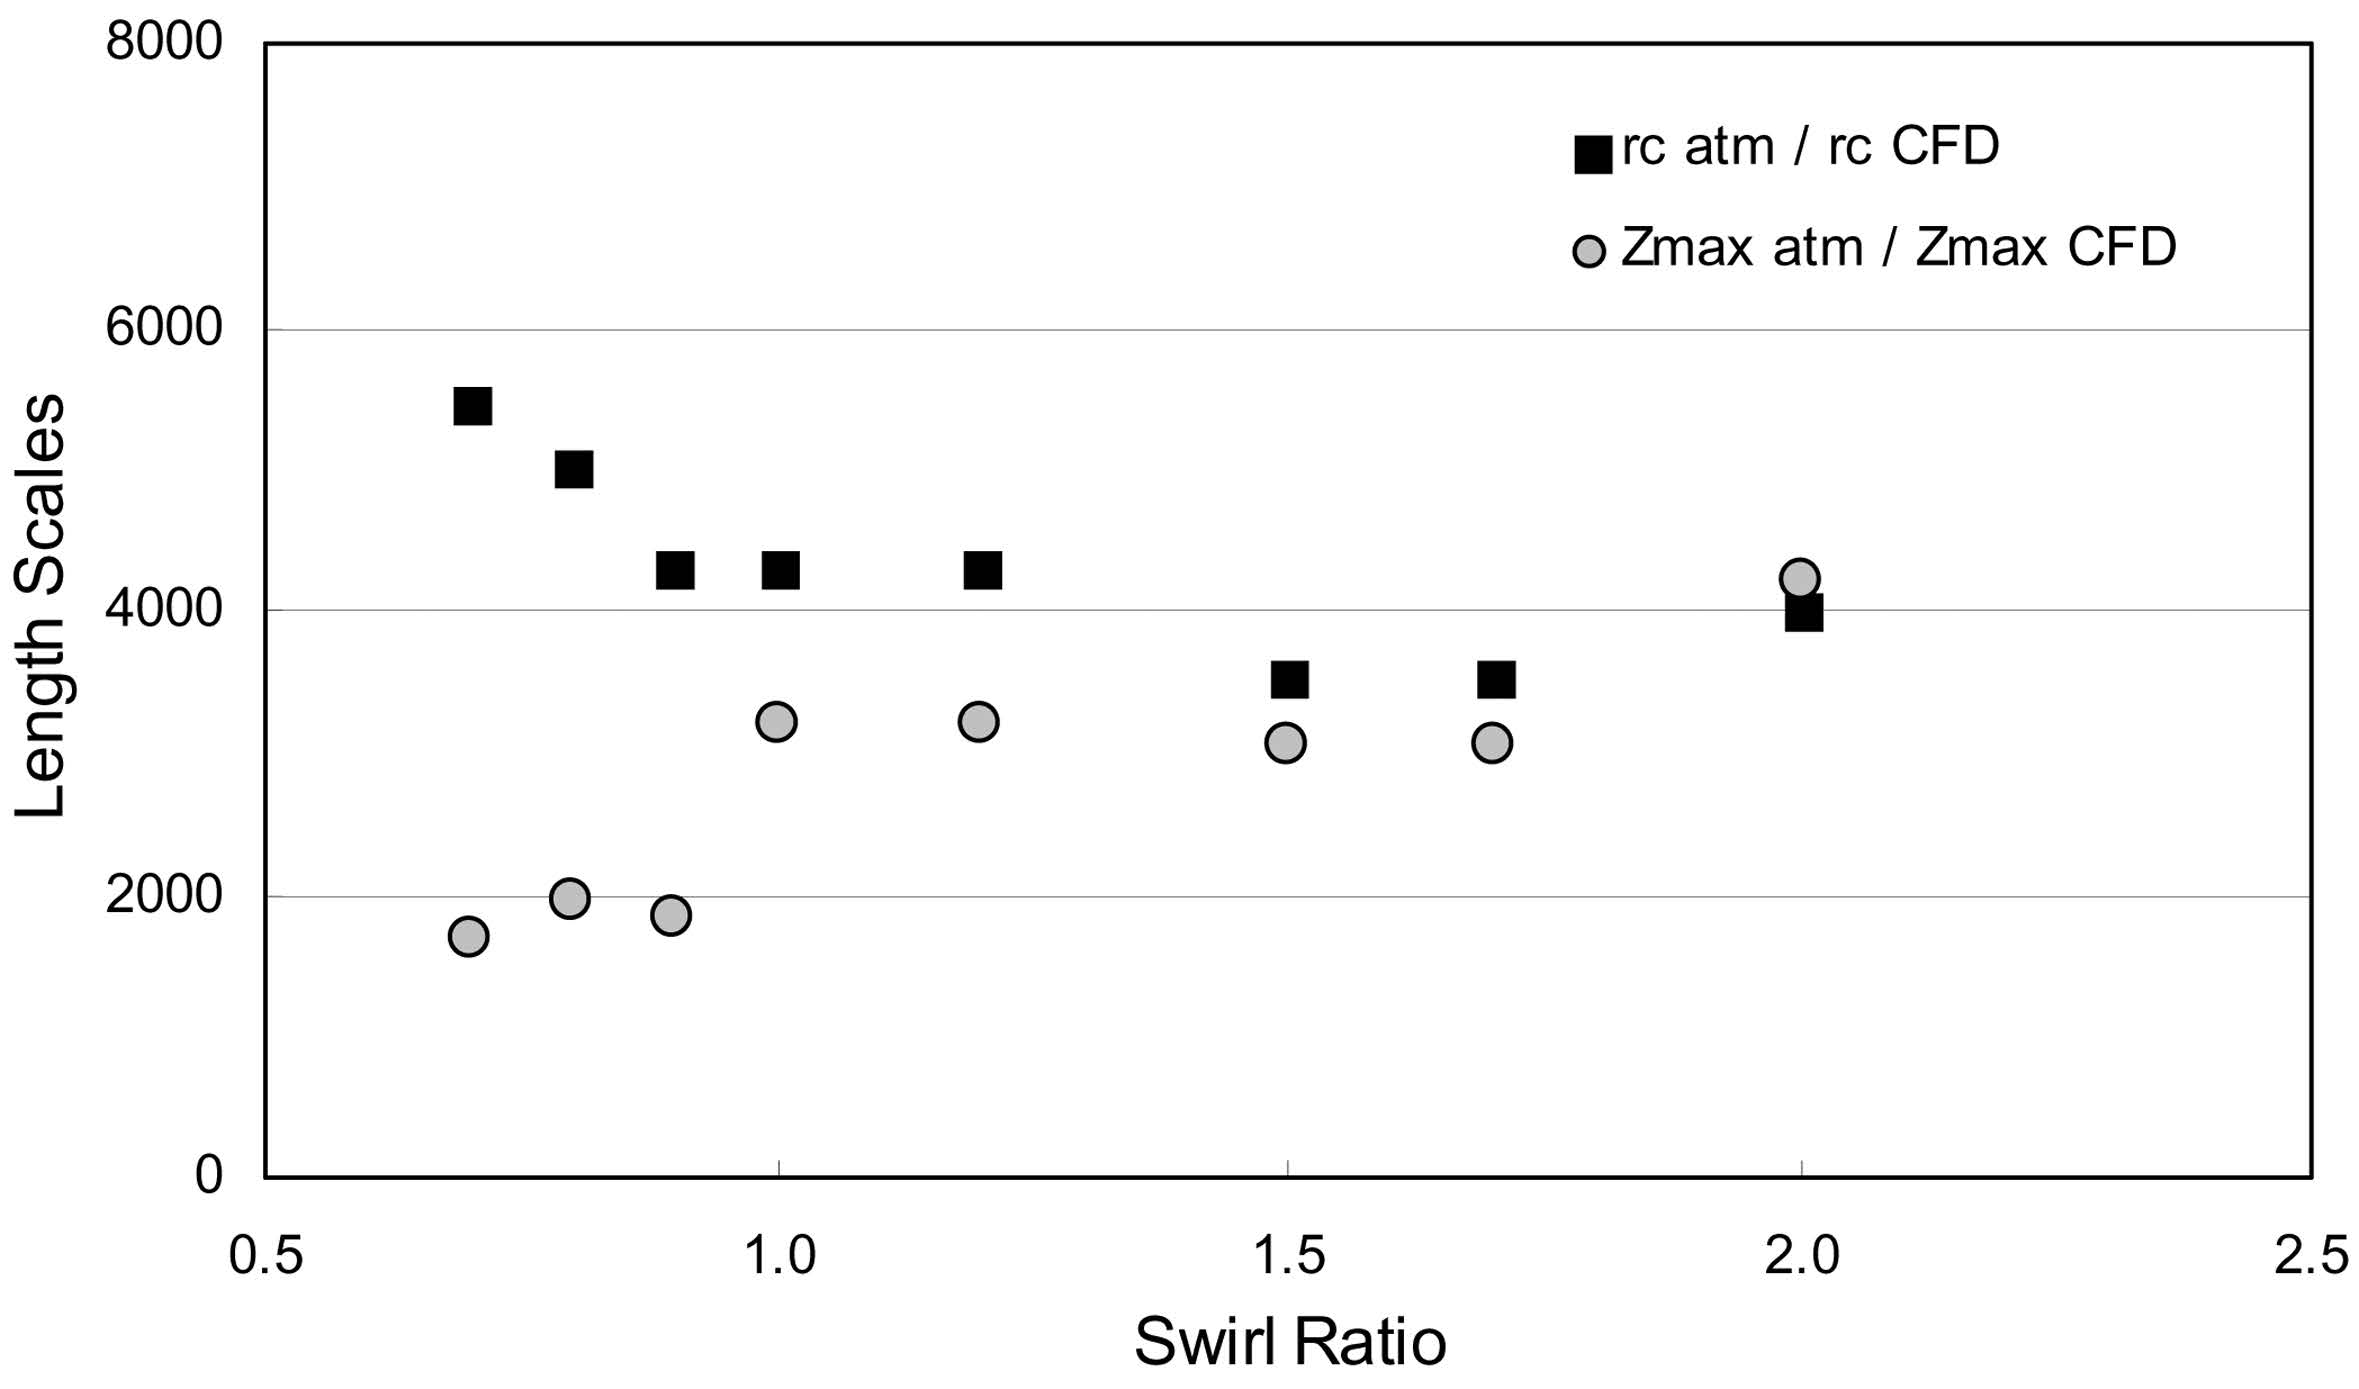
\includegraphics[width=0.8\textwidth]{ls_vs_s.jpg}
	\caption{长度相似比$L_s$随涡流比$S$的变化\cite{hangan2008swirl}}
	\label{fig:Ls-S}
\end{figure}

\subsection{足尺龙卷风风场CFD模拟}\label{sec:full-tornado}

本节利用长度相似比$L_s$和速度相似比$V_s$将缩尺CFD风场转化为足尺龙卷风风场。
首先,将缩尺风场的计算流域(见图\ref{fig:TVC-domain})的底面半径放大为$L_s\times R_0$、
速度入口高度放大为$L_s \times H_0$;
入口边界条件的径向和切向入流速度设置为:
\begin{equation}
	V_r^{\text{Full}}(z) = (V_s V_0)\times\left[z/(L_s z_0)\right]^{1/7}
\end{equation}
\begin{equation}
	V_t^{\text{Full}}(z) = 2 \times S \times V_r^{\text{Full}}(z)
\end{equation}

比较足尺龙卷风风场与Spencer龙卷风实测风场在不同高度处的切向速度沿径向的分布,
见图\ref{fig:cfd-Spencer}所示,二者整体上吻合较好。

\begin{figure}[!htbp]
	\centering
	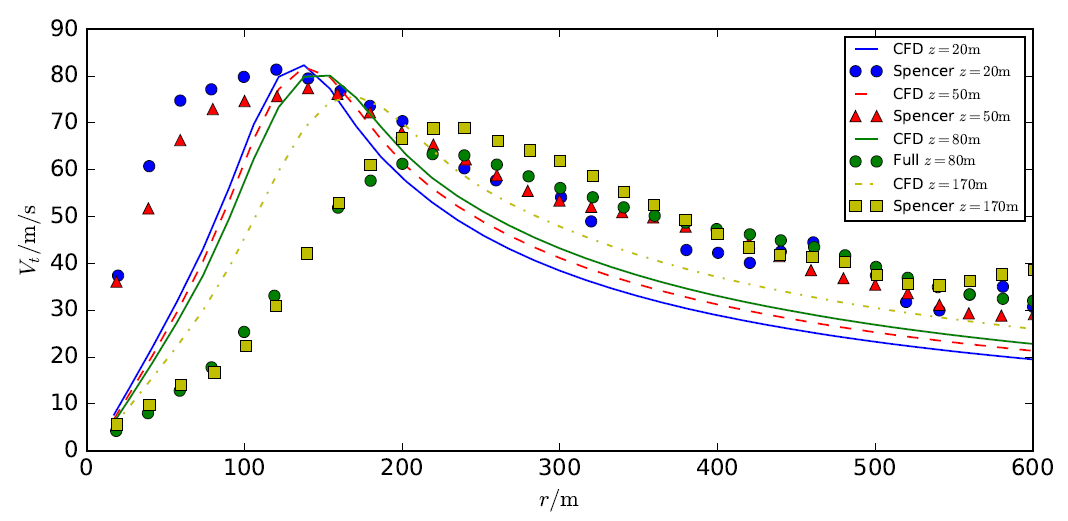
\includegraphics[width=0.8\textwidth]{cfd-vs-Spencer.png}
	\caption{CFD足尺风场与Spencer实测风场切向速度分布比较}
	\label{fig:cfd-Spencer}
\end{figure}
